\subsection{Login}
When a user visits the website they need to decide between logging in using their Feide account, or continue as an anonymous user. At this stage their user-rights level is set to 0, and they can only access the login page. Anonymous users have a user-rights level of 1, and are able to participate in sessions. If the users authenticates with their Feide account, they are assigned a user-rights level depending on their admin status. A normal user with no special rights will get their level set to 2. Level 3 is used for student assistants. Admins (lecturers, professors, ...) are assigned level 4. Users with a user-rights level above 1 are able to see statistics about sessions they have participated in. Student assistants (level 3) currently not implemented. The ability for a admin to add student assistants is added, but at the moment they will not the ability to create, edit and host sessions with questions. Admins will have the highest rights on the website. They will be able to create, edit and delete courses. They will also be able to add other admins or student assistants to a course. Admins will also be able to see and remove other admins and student assistants from a course. Admins will not be able to see other courses that they are not admins for, but will get an error if they try to create a new course with the same information.
\subsubsection{Implementation}
\begin{figure}[h]
    \centering
    \begin{subfigure}{0.45\linewidth}
        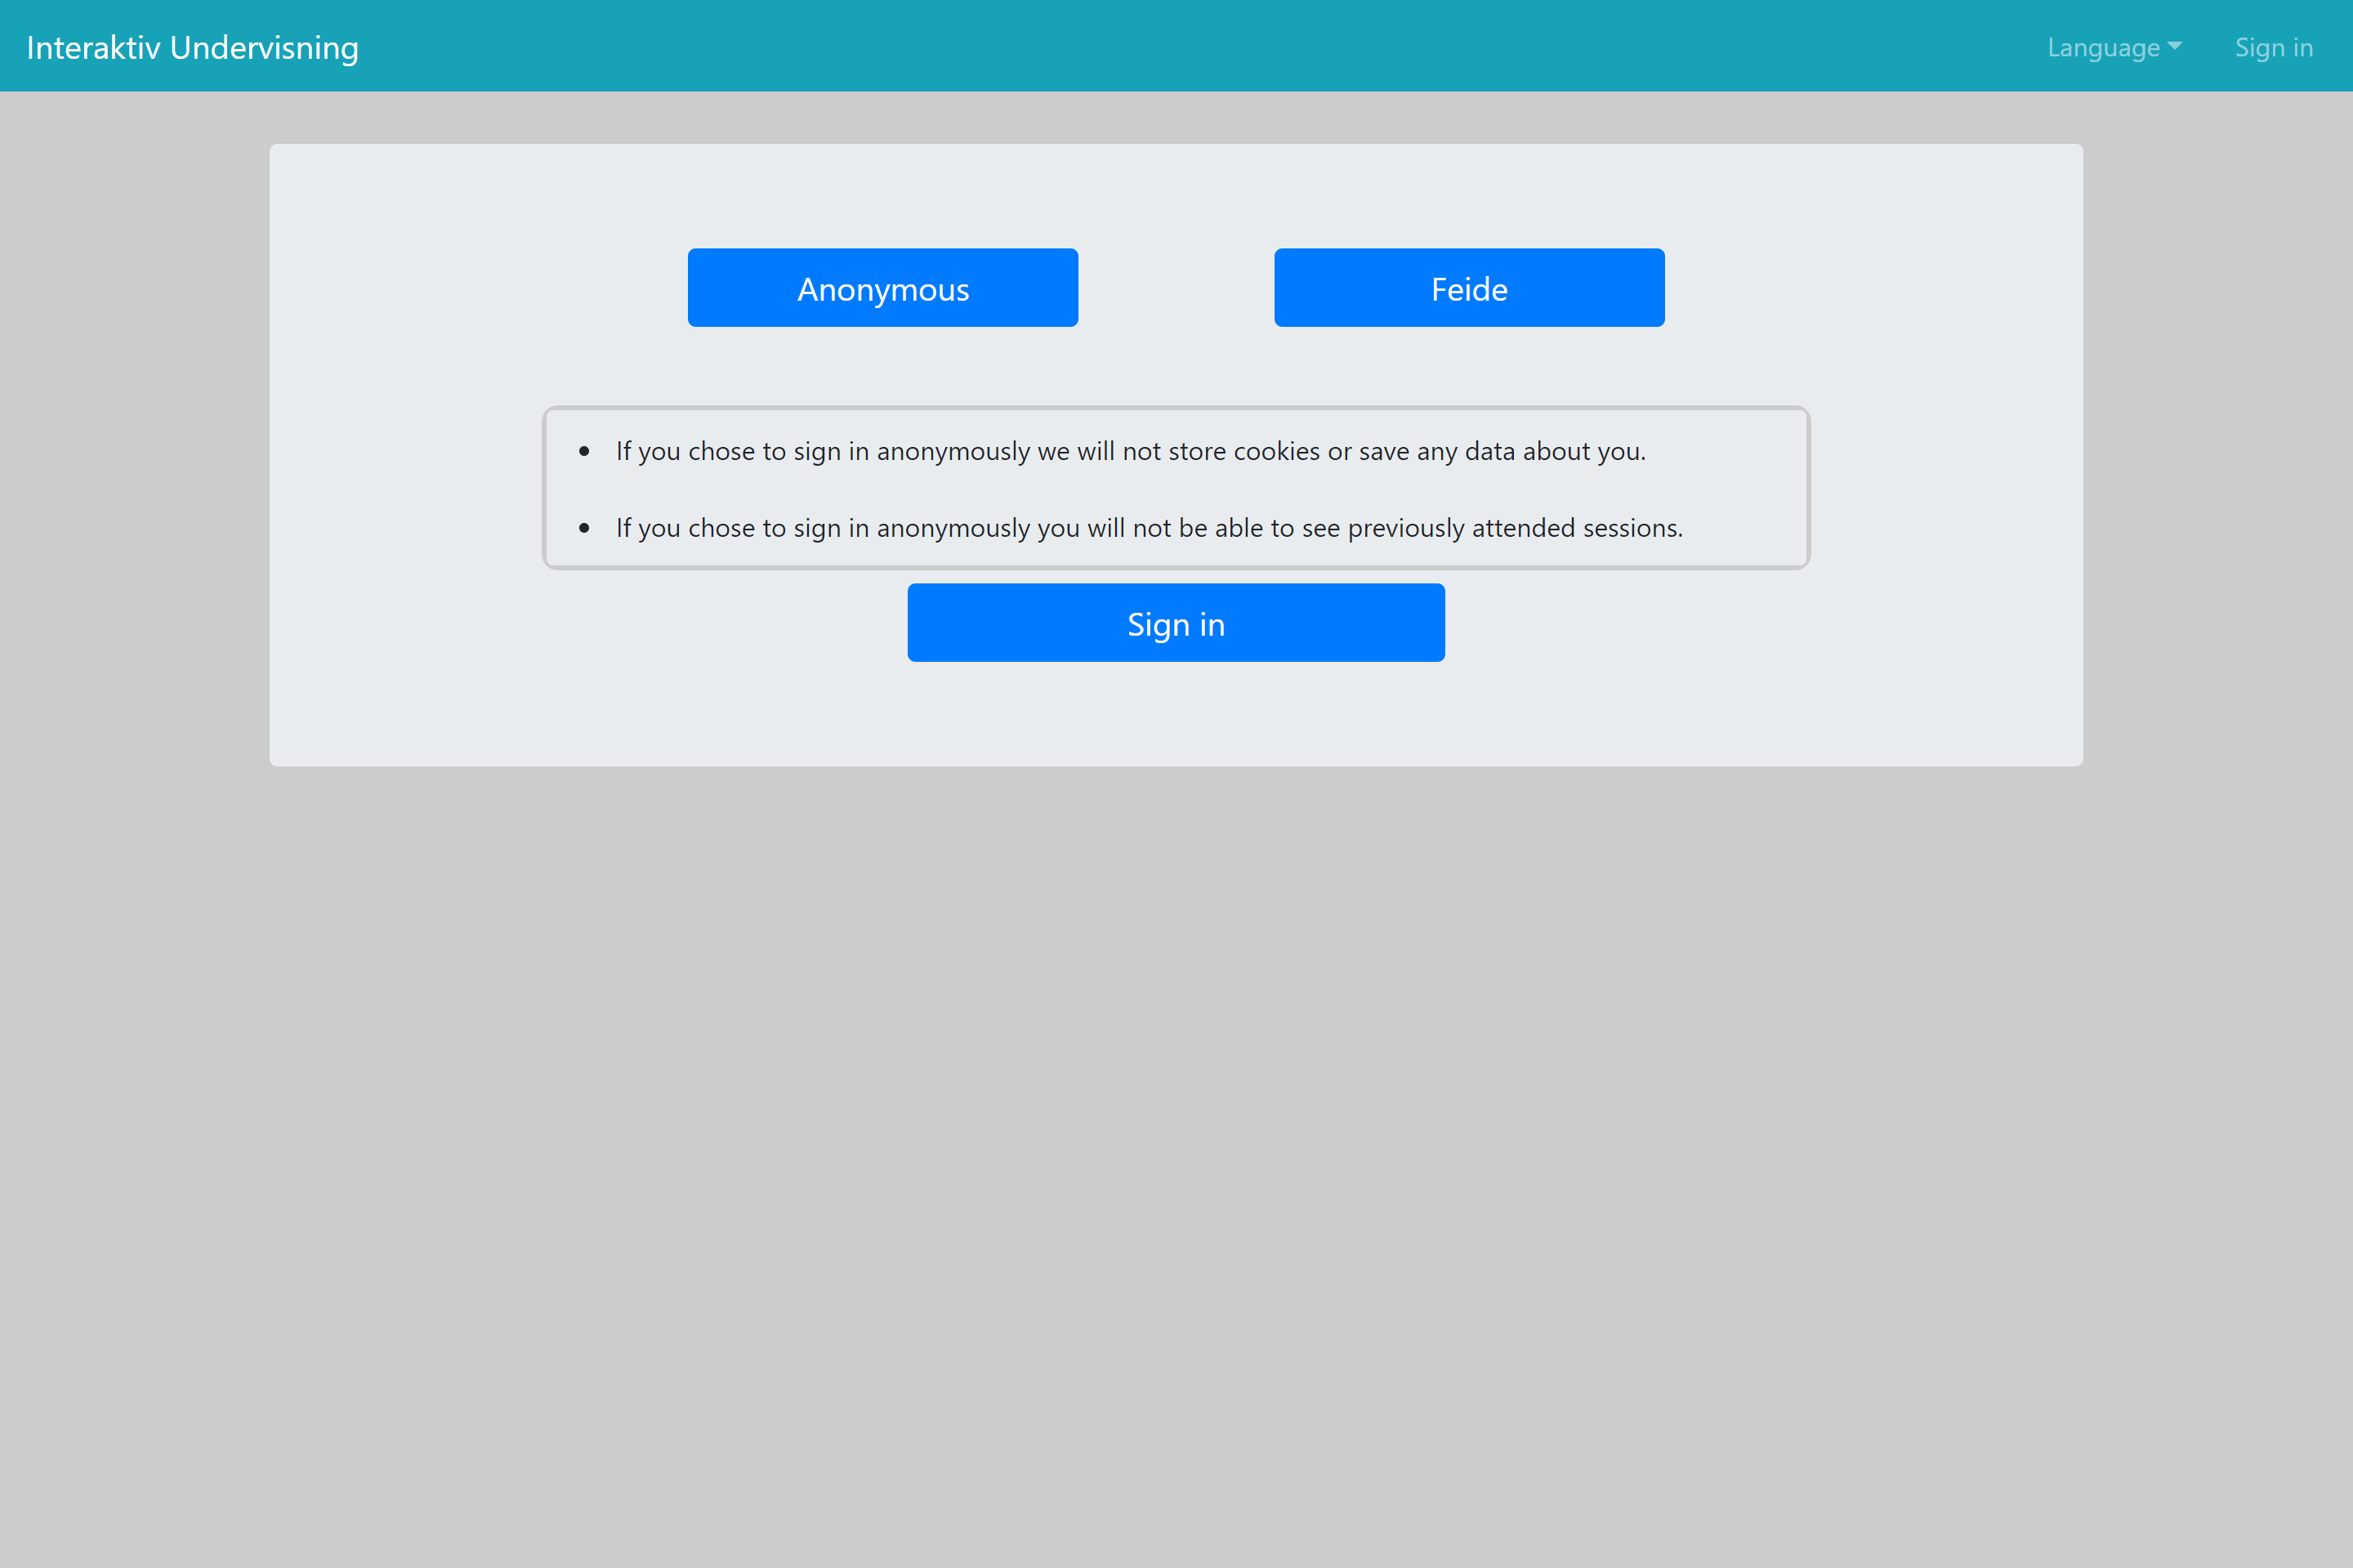
\includegraphics[width=\linewidth]{loginPageAnonymously}
        \caption{This is how the login page looks when anonymously is selected.}
        \label{fig:loginPageAnonoumsly}
    \end{subfigure}
    \begin{subfigure}{0.45\linewidth}
        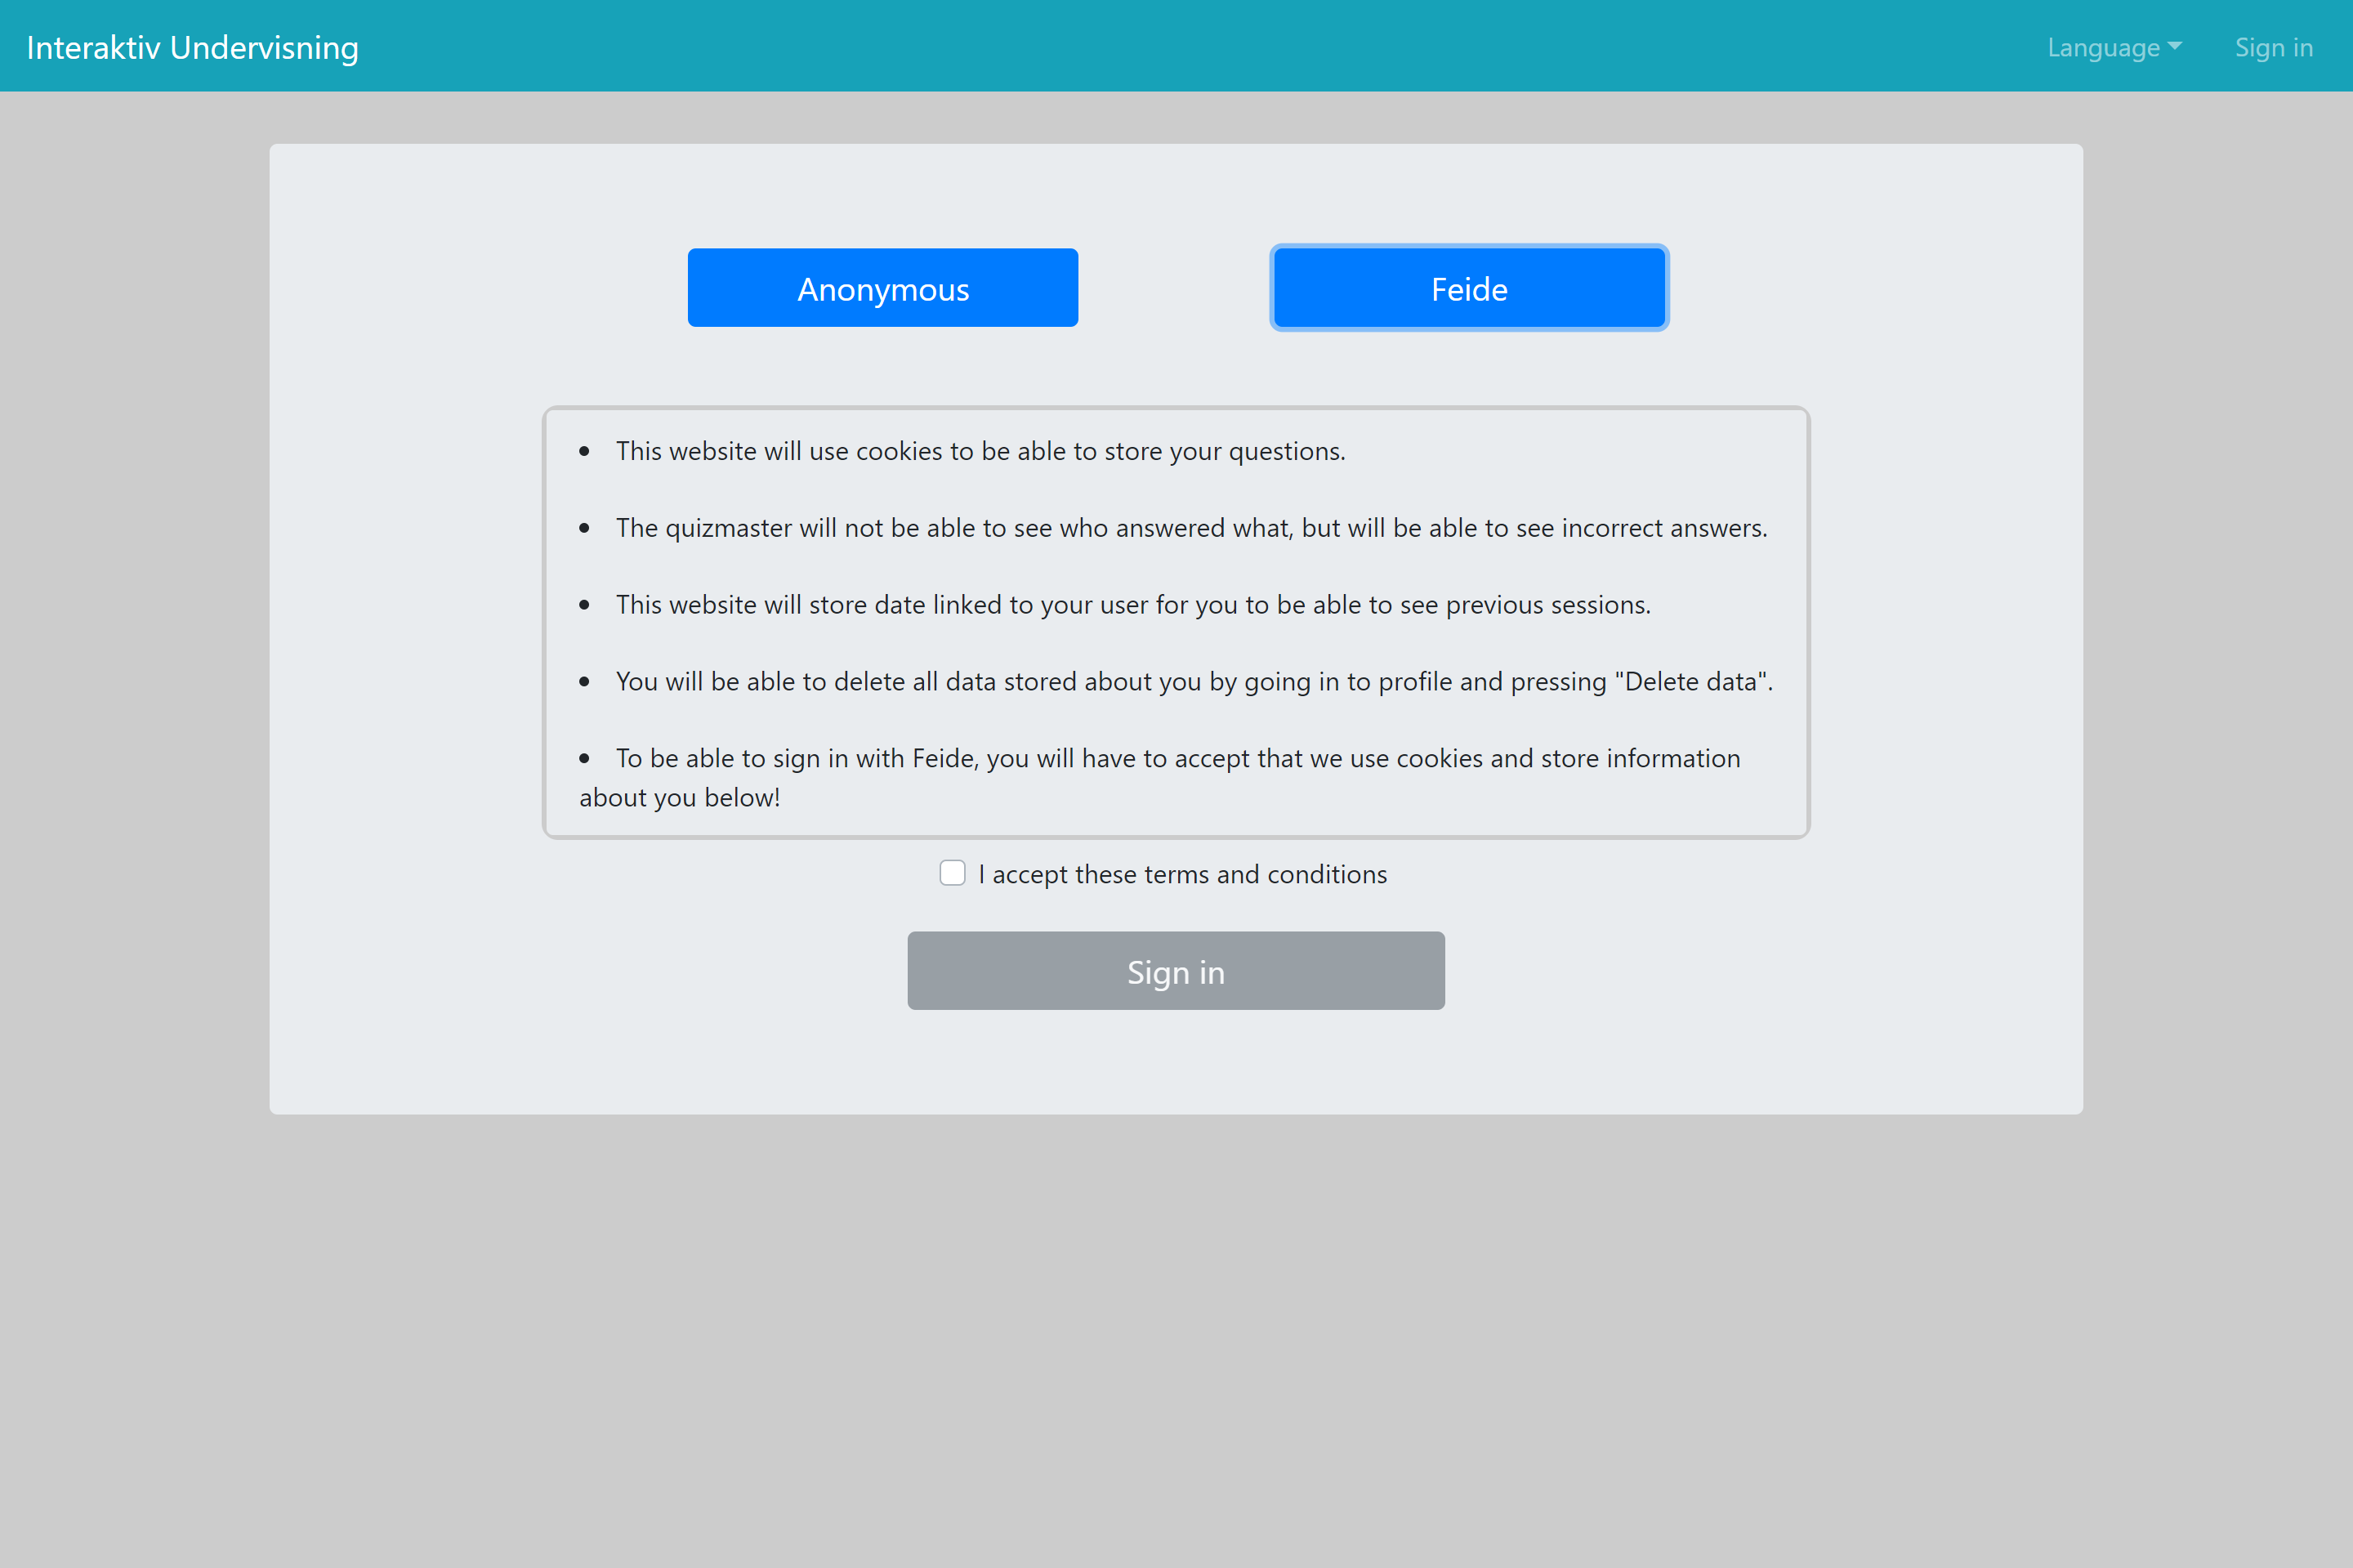
\includegraphics[width=\linewidth]{loginPageFeide}
        \caption{This is how the login page looks when feide is picked.}
        \label{fig:loginPageFeide}
    \end{subfigure}
    \caption{Login Page}
    \label{fig:loginPage}
\end{figure}
\noindent
If a user wants to be anonymous,\cite[][]{VUE:DOC} their user-rights level is first set to 1. They are then redirected to the client page. Since we have decided that an anonymous user shouldn't be tracked or have any information stored about them, they will be limited to only clicking on buttons on the page to navigate. Any attempts to reload the page or go dirrectly to a URL will result in the user getting redirected to the 401 error message indicating that the user isn't authenticated to view this part of the web app. All answers that are sent in by a anonymous user will be stored in the database for the lecturer to view, but there will be no link between the user that answered and the answer that is stored. So all answers from anonymously signed in users will link to the same user in the database.
\\[11pt]
If the user clicks on the Feide login button and accepts the terms, a HTTP POST request is sent to /login/feide. When the server recieves the request, it is passed on to PassportJS's authenticate function. The authenticate function redirects the user to an external site for authentication, before redirecting them back to the specificed callback URL on our site. The authenticate function takes an argument telling it where and how to redirect the user, this is called a strategy. The /login/feide route uses the "passport-openid-connect" strategy to connect to UNINETT's Dataporten authentication servers. If the user successfully login with their Feide account they are redirected back to /login/callback/feide. This route uses the PassportJS authenticate function to exchange the access code with an access token which is then passed on to our route handler. The handler reads the HTTP request to get information about their Feide account. This information is used to check the database and create a in-memory user object which the server uses to decide what the user is allowed to do on the server. The user is finally redirected to the /client route where they can join a session. The server also sends a cookie for feide users so that they will stay authenticated in for 1 day, and during this time there is no need for the user to reauthenticate with feide. When a feide user signs out, the cookie is deleted. Since the web app is designed to be used on campus at UiS users are stored in-memory when they are signed in and active on the web app, but this will result in problems if the app is scaled up to more users.
\\[11pt]
The way the database and the paths are designed it should be easy to add in more sign in option for a user, such as Google, Facebook, etc. The way the user right system is designed, only feide users could become admins or student assistants. When the server first startes the site will have zero admins, but there is a variable in the environment file where admins can be stated. This way will bypass the normal way to add an admin via the admin site.